% !TeX program = pdfLaTeX
\documentclass[12pt]{article}
\usepackage{amsmath}
\usepackage{graphicx,psfrag,epsf}
\usepackage{enumerate}
\usepackage{natbib}
\usepackage{textcomp}
\usepackage[hyphens]{url} % not crucial - just used below for the URL
\usepackage{hyperref}
\providecommand{\tightlist}{%
  \setlength{\itemsep}{0pt}\setlength{\parskip}{0pt}}

%\pdfminorversion=4
% NOTE: To produce blinded version, replace "0" with "1" below.
\newcommand{\blind}{0}

% DON'T change margins - should be 1 inch all around.
\addtolength{\oddsidemargin}{-.5in}%
\addtolength{\evensidemargin}{-.5in}%
\addtolength{\textwidth}{1in}%
\addtolength{\textheight}{1.3in}%
\addtolength{\topmargin}{-.8in}%

%% load any required packages here


\usepackage{color}
\usepackage{fancyvrb}
\newcommand{\VerbBar}{|}
\newcommand{\VERB}{\Verb[commandchars=\\\{\}]}
\DefineVerbatimEnvironment{Highlighting}{Verbatim}{commandchars=\\\{\}}
% Add ',fontsize=\small' for more characters per line
\usepackage{framed}
\definecolor{shadecolor}{RGB}{248,248,248}
\newenvironment{Shaded}{\begin{snugshade}}{\end{snugshade}}
\newcommand{\AlertTok}[1]{\textcolor[rgb]{0.94,0.16,0.16}{#1}}
\newcommand{\AnnotationTok}[1]{\textcolor[rgb]{0.56,0.35,0.01}{\textbf{\textit{#1}}}}
\newcommand{\AttributeTok}[1]{\textcolor[rgb]{0.77,0.63,0.00}{#1}}
\newcommand{\BaseNTok}[1]{\textcolor[rgb]{0.00,0.00,0.81}{#1}}
\newcommand{\BuiltInTok}[1]{#1}
\newcommand{\CharTok}[1]{\textcolor[rgb]{0.31,0.60,0.02}{#1}}
\newcommand{\CommentTok}[1]{\textcolor[rgb]{0.56,0.35,0.01}{\textit{#1}}}
\newcommand{\CommentVarTok}[1]{\textcolor[rgb]{0.56,0.35,0.01}{\textbf{\textit{#1}}}}
\newcommand{\ConstantTok}[1]{\textcolor[rgb]{0.00,0.00,0.00}{#1}}
\newcommand{\ControlFlowTok}[1]{\textcolor[rgb]{0.13,0.29,0.53}{\textbf{#1}}}
\newcommand{\DataTypeTok}[1]{\textcolor[rgb]{0.13,0.29,0.53}{#1}}
\newcommand{\DecValTok}[1]{\textcolor[rgb]{0.00,0.00,0.81}{#1}}
\newcommand{\DocumentationTok}[1]{\textcolor[rgb]{0.56,0.35,0.01}{\textbf{\textit{#1}}}}
\newcommand{\ErrorTok}[1]{\textcolor[rgb]{0.64,0.00,0.00}{\textbf{#1}}}
\newcommand{\ExtensionTok}[1]{#1}
\newcommand{\FloatTok}[1]{\textcolor[rgb]{0.00,0.00,0.81}{#1}}
\newcommand{\FunctionTok}[1]{\textcolor[rgb]{0.00,0.00,0.00}{#1}}
\newcommand{\ImportTok}[1]{#1}
\newcommand{\InformationTok}[1]{\textcolor[rgb]{0.56,0.35,0.01}{\textbf{\textit{#1}}}}
\newcommand{\KeywordTok}[1]{\textcolor[rgb]{0.13,0.29,0.53}{\textbf{#1}}}
\newcommand{\NormalTok}[1]{#1}
\newcommand{\OperatorTok}[1]{\textcolor[rgb]{0.81,0.36,0.00}{\textbf{#1}}}
\newcommand{\OtherTok}[1]{\textcolor[rgb]{0.56,0.35,0.01}{#1}}
\newcommand{\PreprocessorTok}[1]{\textcolor[rgb]{0.56,0.35,0.01}{\textit{#1}}}
\newcommand{\RegionMarkerTok}[1]{#1}
\newcommand{\SpecialCharTok}[1]{\textcolor[rgb]{0.00,0.00,0.00}{#1}}
\newcommand{\SpecialStringTok}[1]{\textcolor[rgb]{0.31,0.60,0.02}{#1}}
\newcommand{\StringTok}[1]{\textcolor[rgb]{0.31,0.60,0.02}{#1}}
\newcommand{\VariableTok}[1]{\textcolor[rgb]{0.00,0.00,0.00}{#1}}
\newcommand{\VerbatimStringTok}[1]{\textcolor[rgb]{0.31,0.60,0.02}{#1}}
\newcommand{\WarningTok}[1]{\textcolor[rgb]{0.56,0.35,0.01}{\textbf{\textit{#1}}}}

% Pandoc citation processing

\usepackage{xcolor, soul, xspace, float, subfig, lineno, setspace, fancyhdr}
\linenumbers
\pagestyle{fancy}
\fancyhead[LO,LE]{forestecology R package}
\renewcommand{\sectionmark}[1]{\markright{#1}{}}

\begin{document}


\def\spacingset#1{\renewcommand{\baselinestretch}%
{#1}\small\normalsize} \spacingset{1}


%%%%%%%%%%%%%%%%%%%%%%%%%%%%%%%%%%%%%%%%%%%%%%%%%%%%%%%%%%%%%%%%%%%%%%%%%%%%%%

\if0\blind
{
  \title{\bf The forestecology R package for fitting and assessing nieghborhood
models of the effect of interspecific competition on the growth of trees}

  \author{
        Albert Y. Kim \thanks{Assistant Professor, Statistical \& Data Sciences, Smith College,
Northampton, MA 01063 (e-mail:
\href{mailto:akim04@smith.edu}{\nolinkurl{akim04@smith.edu}}).} \\
    Program in Statistical \& Data Sciences, Smith College\\
     and \\     David N. Allen \\
    Biology Department, Middlebury College\\
     and \\     Simon P. Couch \\
    Mathematics Department, Reed College\\
      }
  \maketitle
} \fi

\if1\blind
{
  \bigskip
  \bigskip
  \bigskip
  \begin{center}
    {\LARGE\bf The forestecology R package for fitting and assessing nieghborhood
models of the effect of interspecific competition on the growth of trees}
  \end{center}
  \medskip
} \fi

\bigskip
\begin{abstract}
1. Neighborhood competition models are powerful tools to measure the
effect of interspecific competition. Statistical methods to ease the
application of these models are currently lacking.\\
2. We present the \texttt{forestecology} package providing methods to i)
specify neighborhood competition models, ii) evalulate the effect of
competitor species identity using permutation tests, and iii) measure
model performance using spatial cross-validation. Following
\citet{allen_permutation_2020}, we implement a Bayesian linear
regression neighborhood competition model.\\
3. We demonstrate the package's functionality using data from the
Smithsonian Conservation Biology Institute's large forest dynamics plot,
part of the ForestGEO global network of reseach sites. Given ForestGEO's
data collection protocols and data formatting standards, the package was
designed with cross-site compatibility in mind. We highlight the
importance of spatial cross validation when interpreting model
results.\\
4. The package features i) \texttt{tidyverse}-like structure whereby
verb-named functions can be modularly ``piped'' in sequence, ii)
functions with standardized inputs/outputs of simple features
\texttt{sf} package class, and iii) an S3 object-oriented implementation
of the Bayesian linear regression model. These three facts allow for
clear articulation of all the steps in the sequence of analysis and easy
wrangling and visualization of the geospatial forestry data.
Furthermore, while the package only has Bayesian linear regression
implemented, the package was designed with extensibility to other
methods in mind.
\end{abstract}

\noindent%
{\it Keywords:} forest ecology, interspecific competition, neigbhorhood competition,
tree growth, R, ForestGEO, spatial cross validation
\vfill

\newpage
\spacingset{1.45} % DON'T change the spacing!

\doublespacing

\hypertarget{introduction}{%
\section{Introduction}\label{introduction}}

Repeat-censused forest plots offer excellent opportunities to test
neighborhood models of the effect of competition on the growth of trees
(\citet{canham_neighborhood_2004}). Neighborhood models of competition
have been used to: test whether the species identity of a competitor
matters (\citet{uriarte_spatially_2004}); measure species-specific
competition coefficients (\citet{das_effect_2012}
\citet{tatsumi_estimating_2016}); test competing models to see what
structures competitive interactions, e.g.~traits or phylogeny
(\citet{allen_permutation_2020}; \citet{uriarte_trait_2010}); and inform
selective logging practices (\citet{canham_neighborhood_2006}). Although
these are well-described methods, no methods are currently available for
their easy application. Here we address this in an R package. We largely
follow the methods presented in \citet{allen_permutation_2020}. The
package is written to model stem radial growth between two censuses
based on neighborhood competition.

\citet{allen_permutation_2020} considers the following model: Let
\(i = 1, \ldots, n_j\) index all \(n_j\) trees of ``focal'' species
group \(j\); let \(j = 1, \ldots, J\) index all \(J\) focal species
groups; and let \(k = 1, \ldots, K\) index all \(K\) ``competitor''
species groups. We model the average annual growth in diameter
\(y_{ij}\) (in centimeters per year) of the \(i^{th}\) tree of focal
species group \(j\) as a linear model \(f\) of the covariates
\(\vec{x}_{ij}\)

\begin{equation}
\label{eq:model}
y_{ij} = f(\vec{x}_{ij}) + \epsilon_{ij} = \beta_{0,j} + \beta_{\text{dbh},j} \cdot \text{dbh}_{ij} + \sum_{k=1}^{K} \lambda_{jk} \cdot \text{BA}_{ijk} + \epsilon_{ij}
\end{equation}

where \(\beta_{0,j}\) is the diameter-independent growth rate for group
\(j\); \(\text{dbh}_{ij}\) is the diameter at breast height (in
centimeters) of the focal tree at the earlier census;
\(\beta_{\text{dbh},j}\) is the amount of the growth rate changed
depending on diameter for group \(j\); \(\text{BA}_{ijk}\) is the sum of
the basal area of all trees of competitor species group \(k\);
\(\lambda_{jk}\) is the change in growth for individuals of group \(j\)
from nearby competitors of group \(k\); and \(\epsilon_{ij}\) is a
random error term distributed \(\text{Normal}(0, \sigma^2)\). They
estimate all parameters via Bayesian linear regression while exploiting
Normal/Inverse Gamma conjugacy to derive closed-form solutions to all
posterior distributions via linear algebra\footnote{See S1 Appendix of
  \citet{allen_permutation_2020}, available at
  \url{https://doi.org/10.1371/journal.pone.0229930.s004}}. These
closed-form solutions for the posterior distributions are in contrast to
approximations of all posteriors via computationally expensive Markov
Chain Monte Carlo algorithms.

In order to evaluate whether competitor species identity matters,
\citet{allen_permutation_2020} run a permutation test where under the
null hypothesis the species identity of all competitors of a focal tree
can be permuted/shuffled:

\begin{eqnarray}
\label{eq:permutation-hypothesis-test}
&&H_0: \lambda_{jk} = \lambda_{j} \mbox{ for all } k = 1, \ldots, K\\
\text{vs.}&&H_A: \text{at least one } \lambda_{jk} \mbox{ is different}
\end{eqnarray}

where the null hypothesis \(H_0\) reflects a hypothesis of no species
grouping-specific effects of competition while the alternative
hypothesis \(H_A\) reflects a hypothesis of species grouping-specific
effects of competition. Furthermore, in order to account for the spatial
autocorrelation inherent to forest data in their estimates of
out-of-sample model error, \citet{allen_permutation_2020} use spatial
cross-validation. Estimates of model error that do not account for this
spatial dependency tend to underestiamte the true model error
\citep{roberts_cross-validation_2017}.

We introduce the \texttt{forestecology} R package providing methods and
data for forest ecology model fitting and assessment, available on CRAN
(\url{https://cran.r-project.org/web/packages/forestecology/index.html})
with the corresponding source code available on GitHub
(\url{https://github.com/rudeboybert/forestecology}). The package
implements all aspects of the model in Equation \ref{eq:model}: model
fitting and generating fitted/predicted values, evaluating the effect of
competitor species identity using permutation tests, and evaluating
model performance using spatial cross-validation.

The package designed with ``tidy'' design principles in mind
\citep{wickham_welcome_2019}. Much like many of the \texttt{tidyverse}
component packages, \texttt{forestecology} is designed with verb-named
functions that can be modularly composed in sequence using the pipe
\texttt{\%\textgreater{}\%} operator \citep{bache_pipe_2020}. As we
articulate in Section \ref{casestudy}, these functions delineate the key
steps in our analysis sequence. Furthermore, the inputs and outputs of
nearly all of our functions use the same ``simple features for R'' data
structures as implemented in the \texttt{sf} package for standardized
support for spatial vector data \citep{pebesma_simple_2018}. The
\texttt{sf} package is a \texttt{tidyverse}-friendly evolution of the
\texttt{sp} package of classes and methods for spatial data in R
\citep{pebesma_sp_2005}. As such, wrangling and visualization spatial
data such as ours becomes much easier.

Currently the package only implements the Bayesian linear regression
model of tree growth based on neighborhood competition detailed in
Equation \ref{eq:model}. As we demonstrate in Section
\ref{model-fit-predict} however, the fitting of this model is
self-contained in a single function \texttt{comp\_bayes\_lm()}. This
function returns an object of S3 class type \texttt{comp\_bayes\_lm}
with generic methods implemented for \texttt{print()} to inspect the
output, \texttt{predict()} to generate fitted/predicted values, and
\texttt{ggplot2::autoplot()} to visualize all results. Therefore the
package can be modularly extended to fit other models as long as they
are coded into a function similar type as \texttt{comp\_bayes\_lm()} as
has equivalent generic methods implemented.

We present a case-study of the \texttt{forestecology} package's use on
data from the Smithsonian Conservation Biology Institute's (SCBI) large
forest dynamics plot in Front Royal, Virginia, USA in Section
\ref{casestudy}, which is part of the ForestGEO global network of
research sites
\citep[\citet{andersonteixeira_ctfs-forestgeo_2015}]{bourg_initial_2013}.
The package is designed with ForestGEO plot data in mind, but we
envision that it could easily be modified to work with data from other
forest plots, e.g.~the US Forest Service Forest Inventory and Analysis
plots or more generally to model interactions of any community of mapped
sessile organisms \citep{smith_forest_2002}.

\hypertarget{casestudy}{%
\section{forestecology workflow: a case study}\label{casestudy}}

We demonstrate the \texttt{forestecology} package's functionality on
data from the Smithsonian Conservation Biology Institute (SCBI) large
forest dynamics plot, located at the Smithsonian's National Zoo and
Conservation Biology Institute in Front Royal, VA, USA
\citep{bourg_initial_2013}. The 25.6 ha (640 x 400 m) plot is located at
the intersection of three of the major physiographic provinces of the
eastern US---the Blue Ridge, Ridge and Valley, and Piedmont
provinces---and is adjacent to the northern end of Shenandoah National
Park. The forest type is typical mature secondary eastern mixed
deciduous forest, with a canopy dominated by tulip poplar
(\emph{Liriodendron tulipifera}), oaks (\emph{Quercus} spp.), and
hickories (\emph{Carya} spp.), and an understory composed mainly of
spicebush (\emph{Lindera benzoin}), paw-paw (\emph{Asimina triloba}),
American hornbeam (\emph{Carpinus caroliniana}), and witch hazel
(\emph{Hamamelis virginiana}) \citep{bourg_initial_2013}.

The \texttt{forestecology} package has the following ecological goals:
1) to evaluate the effect of competitor species identity using
permutation tests and 2) to evaluate model performance using spatial
cross-validation. To achieve these goals, we outline a basic analysis
sequence comprising of these four main steps:

\begin{enumerate}
\def\labelenumi{\arabic{enumi}.}
\tightlist
\item
  Compute the growth of stems based on two censuses.
\item
  Add spatial information:

  \begin{enumerate}
  \def\labelenumii{\arabic{enumii}.}
  \tightlist
  \item
    Define a buffer region of trees.
  \item
    Add spatial cross-validation block information.
  \end{enumerate}
\item
  Identify all focal trees and their competitors.
\item
  Apply model, which includes:

  \begin{enumerate}
  \def\labelenumii{\arabic{enumii}.}
  \tightlist
  \item
    Fit model.
  \item
    Compute fitted/predicted values.
  \item
    Visualize posterior distributions.
  \end{enumerate}
\end{enumerate}

We start by loading all necessary packages.

\begin{Shaded}
\begin{Highlighting}[]
\KeywordTok{library}\NormalTok{(tidyverse)}
\KeywordTok{library}\NormalTok{(lubridate)}
\KeywordTok{library}\NormalTok{(sf)}
\KeywordTok{library}\NormalTok{(patchwork)}
\KeywordTok{library}\NormalTok{(forestecology)}
\KeywordTok{library}\NormalTok{(blockCV)}
\end{Highlighting}
\end{Shaded}

\hypertarget{step-1-compute-the-growth-of-trees-based-on-census-data-compute-growth}{%
\subsection{Step 1: Compute the growth of trees based on census data
\{compute-growth\}}\label{step-1-compute-the-growth-of-trees-based-on-census-data-compute-growth}}

The first step in the our analysis sequence is to compute the growth of
trees using data from two censuses. The \texttt{compute\_growth()}
function computes average annual growth assuming census data that
roughly follows ForestGEO standards. Despite such standards, minor
variations will still exist between sites, thereby necessitating some
data wrangling and checking. For example, the SCBI site records all
diameters at breast height (DBH) in millimeters
\citep{bourg_initial_2013}, whereas the Michigan Big Woods site records
them in centimeters \citep{allen_michigan_2020}.

We load both 2008 and 2014 SCBI census data \texttt{.csv} files as they
existed on GitHub on November 20, 2020
\citep{gonzalez-akre_scbi-forestgeoscbi-forestgeo-data_2020}. After
selecting only the relevant variables, we perform a few additional data
wrangling steps: convert the character variable with the date of
measurement to be of explicit type \texttt{date}, convert DBH to be in
centimeters\footnote{A rule of thumb to determine the units of DBH is to
  check if the smallest non-zero and non-missing measurement is 1 or 10.
  If the former, then centimeters. If the later, then millimeters. This
  is because ForestGEO protocols state that only trees with DBH greater
  or equal to 1cm should be included in censuses.} Furthermore, in order
to speed up computation for purposes of this example, we only consider a
9 ha subsection of the 25.6 ha of the SCBI site: \texttt{gx} from 0--300
instead of 0--400 and \texttt{gy} from 300--600 instead of 0--640.

\begin{Shaded}
\begin{Highlighting}[]
\NormalTok{census_}\DecValTok{2013}\NormalTok{_scbi <-}\StringTok{ }\KeywordTok{read_csv}\NormalTok{(}\StringTok{"scbi.stem2.csv"}\NormalTok{) }\OperatorTok
\StringTok{  }\KeywordTok{select}\NormalTok{(stemID, sp, }\DataTypeTok{date =}\NormalTok{ ExactDate, gx, gy, dbh, codes, status) }\OperatorTok
\StringTok{  }\KeywordTok{mutate}\NormalTok{(}
    \DataTypeTok{date =} \KeywordTok{mdy}\NormalTok{(date),}
    \DataTypeTok{dbh =} \KeywordTok{as.numeric}\NormalTok{(dbh)}\OperatorTok{/}\DecValTok{10}
\NormalTok{  ) }\OperatorTok
\StringTok{  }\KeywordTok{filter}\NormalTok{(gx }\OperatorTok{<}\StringTok{ }\DecValTok{300}\NormalTok{, }\KeywordTok{between}\NormalTok{(gy, }\DecValTok{300}\NormalTok{, }\DecValTok{600}\NormalTok{))}

\NormalTok{census_}\DecValTok{2018}\NormalTok{_scbi <-}\StringTok{ }\KeywordTok{read_csv}\NormalTok{(}\StringTok{"scbi.stem3.csv"}\NormalTok{) }\OperatorTok
\StringTok{  }\KeywordTok{select}\NormalTok{(stemID, sp, }\DataTypeTok{date =}\NormalTok{ ExactDate, gx, gy, dbh, codes, status) }\OperatorTok
\StringTok{  }\KeywordTok{mutate}\NormalTok{(}
    \DataTypeTok{date =} \KeywordTok{mdy}\NormalTok{(date),}
    \DataTypeTok{dbh =} \KeywordTok{as.numeric}\NormalTok{(dbh)}\OperatorTok{/}\DecValTok{10}
\NormalTok{  ) }\OperatorTok
\StringTok{  }\KeywordTok{filter}\NormalTok{(gx }\OperatorTok{<}\StringTok{ }\DecValTok{300}\NormalTok{, }\KeywordTok{between}\NormalTok{(gy, }\DecValTok{300}\NormalTok{, }\DecValTok{600}\NormalTok{))}
\end{Highlighting}
\end{Shaded}

These two data frames are then supplied as arguments to the
\texttt{compute\_growth()} function, along with the \texttt{id} argument
that specifies the variable that uniquely identifies each tree-stem.
Note furthermore that we discard all resprouts in the later census
(those with \texttt{code\ ==\ R}), since we are only interested in the
diameter growth of surviving, and not resprouted, stems.

\begin{Shaded}
\begin{Highlighting}[]
\NormalTok{growth_scbi <-}
\StringTok{  }\KeywordTok{compute_growth}\NormalTok{(}
    \DataTypeTok{census_1 =}\NormalTok{ census_}\DecValTok{2013}\NormalTok{_scbi,}
    \DataTypeTok{census_2 =}\NormalTok{ census_}\DecValTok{2018}\NormalTok{_scbi }\OperatorTok\StringTok{ }\KeywordTok{filter}\NormalTok{(}\OperatorTok{!}\KeywordTok{str_detect}\NormalTok{(codes, }\StringTok{"R"}\NormalTok{)),}
    \DataTypeTok{id =} \StringTok{"stemID"}
\NormalTok{  )}
\NormalTok{growth_scbi}
\CommentTok{## Simple feature collection with 7954 features and 8 fields}
\CommentTok{## geometry type:  POINT}
\CommentTok{## dimension:      XY}
\CommentTok{## bbox:           xmin: 0.2 ymin: 300 xmax: 300 ymax: 600}
\CommentTok{## CRS:            NA}
\CommentTok{## # A tibble: 7,954 x 9}
\CommentTok{##   stemID sp     dbh1 codes1 status  dbh2 codes2 growth   geometry}
\CommentTok{##    <dbl> <fct> <dbl> <chr>  <chr>  <dbl> <chr>   <dbl>    <POINT>}
\CommentTok{## 1      4 nysy  13.6  M      A       14.2 M       0.103 (14.2 428)}
\CommentTok{## 2      5 havi   8.8  M      A        9.6 M;P     0.150  (9.4 436)}
\CommentTok{## 3      6 havi   3.25 NULL   A        4   M       0.140  (1.3 434)}
\CommentTok{## 4     77 qual  65.2  M      A       66   M       0.141 (34.7 307)}
\CommentTok{## 5     79 tiam  47.7  M      A       46.8 M      -0.161   (40 381)}
\CommentTok{## # ... with 7,949 more rows}
\end{Highlighting}
\end{Shaded}

The output \texttt{growth\_scbi} is a single data frame of class
\texttt{sf} that includes variables \texttt{growth}, the average annual
growth in DBH (cm y\textsuperscript{-1}) for all stems that were alive
at both time points, and \texttt{geometry}, the \texttt{sf} package's
encoding of geolocations of type
\texttt{\textless{}POINT\textgreater{}}. In addition the species
variable \texttt{sp} is converted to a factor if it wasn't already by
\texttt{compute\_growth()}.\footnote{In our spatial cross-validation
  algorithm in Section \ref{spatial-cross-validation} issues can occur
  when rare species do not occur in the training set, but then are
  encountered in the test set. This risk is mitigated by representing
  \texttt{sp} as a factor variable, which has a complete list of all
  levels of the categorical variable.} Furthermore, the variables that
should remain unchanged between censuses appear only once, such as
location variables \texttt{gx} and \texttt{gy}; as well as
species-related variables. Variables that should change between censuses
are suffixed with \texttt{1} and \texttt{2} indicating the earlier and
later censuses, such as \texttt{dbh1/dbh2} and \texttt{codes1/codes2}.

Site data that does not align with this convention will need to be
transformed for use with the \texttt{compute\_growth()} function.
However, in the end, all that matters is that the growth of all stems is
saved in a data frame of class \texttt{sf} and, at a minimum, contains
the variable uniquely identifying each stem, \texttt{sp}, \texttt{dbh1},
\texttt{growth}, \texttt{geometry}.

Given that \texttt{growth\_scbi} is of class \texttt{sf}, it can be
easily plotted in \texttt{ggplot2} using the \texttt{geom\_sf()}
geometry as seen in Figure \ref{fig:scbi-trees} where we plot a random
sample of 500 out of the 7954 trees.

\begin{Shaded}
\begin{Highlighting}[]
\KeywordTok{ggplot}\NormalTok{() }\OperatorTok{+}
\StringTok{  }\KeywordTok{geom_sf}\NormalTok{(}\DataTypeTok{data =}\NormalTok{ growth_scbi }\OperatorTok\StringTok{ }\KeywordTok{sample_n}\NormalTok{(}\DecValTok{500}\NormalTok{), }\KeywordTok{aes}\NormalTok{(}\DataTypeTok{size =}\NormalTok{ growth)) }\OperatorTok{+}\StringTok{ }
\StringTok{  }\KeywordTok{scale_size_binned}\NormalTok{(}\DataTypeTok{limits =} \KeywordTok{c}\NormalTok{(}\FloatTok{0.1}\NormalTok{, }\DecValTok{1}\NormalTok{))}
\end{Highlighting}
\end{Shaded}

\begin{figure}

{\centering 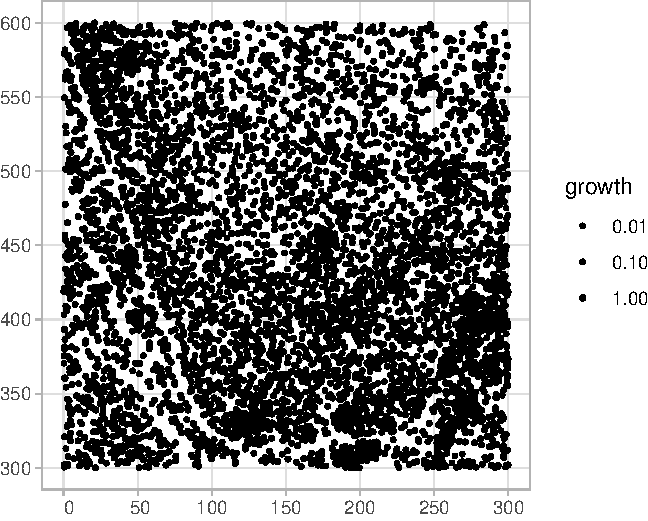
\includegraphics[width=0.66\linewidth]{Figures/scbi-trees-1} 

}

\caption{Compute growth of trees based on census data: Map with growth of a random sample of 500 trees from a 9 ha subsection of the Smithsonian Conservation Biology Institute (SCBI) forest plot.}\label{fig:scbi-trees}
\end{figure}

\hypertarget{spatial-information}{%
\subsection{Step 2: Add spatial information}\label{spatial-information}}

The next step in our analysis sequence is to add additional spatial
information to our main \texttt{growth\_scbi} data frame. The first
element of spatial information we add is a ``buffer region'' to the
periphery of the study region. Since some of our model's explanatory
variables are cumulative (such as competitor basal area), we must ensure
that all trees being modeled are not biased to have different neighbor
structures. This is of concern for trees at the boundary of study
regions, for which all neighbors will not be included in the censused
stems. In order to account for such edge effects, only trees that are
not part of this buffer region, i.e.~are part of the interior of the
study region, will have their growth modeled
\citep{waller_applied_2004}.

Our model of interspecific competition relies on a spatial definition of
who the competitor trees are for focal trees of interest: all trees
within a distance \texttt{comp\_dist} of a focal tree are considered its
competitors (assuming the same units as the \texttt{gx} and \texttt{gy}
location variables). In our case we set this value at 7.5m, a value
informed by other studies \citep[\citet{uriarte_spatially_2004},
\citet{canham_neighborhood_2006}]{canham_neighborhood_2004}. Using this
value along with a manually constructed \texttt{sf} object
representation of the study region's boundary via its vertices, we apply
the \texttt{add\_buffer\_variable()} to our \texttt{growth\_scbi} data
frame to add a \texttt{buffer} boolean variable: all trees who have
\texttt{buffer} set to \texttt{FALSE} will be our focal trees whose
growth will be modeled, whereas those with \texttt{TRUE} will only be
considered as competitor trees whose growth will not.

\begin{Shaded}
\begin{Highlighting}[]
\CommentTok{# Define buffer region using competitive distance range}
\NormalTok{comp_dist <-}\StringTok{ }\FloatTok{7.5}

\NormalTok{study_region_scbi <-}\StringTok{ }\KeywordTok{tibble}\NormalTok{(}
  \DataTypeTok{x =} \KeywordTok{c}\NormalTok{(}\DecValTok{0}\NormalTok{, }\DecValTok{300}\NormalTok{, }\DecValTok{300}\NormalTok{, }\DecValTok{0}\NormalTok{, }\DecValTok{0}\NormalTok{),}
  \DataTypeTok{y =} \KeywordTok{c}\NormalTok{(}\DecValTok{300}\NormalTok{, }\DecValTok{300}\NormalTok{, }\DecValTok{600}\NormalTok{, }\DecValTok{600}\NormalTok{, }\DecValTok{300}\NormalTok{)}
\NormalTok{) }\OperatorTok
\StringTok{  }\KeywordTok{sf_polygon}\NormalTok{()}

\NormalTok{growth_scbi <-}\StringTok{ }\NormalTok{growth_scbi }\OperatorTok
\StringTok{  }\KeywordTok{add_buffer_variable}\NormalTok{(}\DataTypeTok{size =}\NormalTok{ comp_dist, }\DataTypeTok{region =}\NormalTok{ study_region_scbi)}
\end{Highlighting}
\end{Shaded}

The second element of spatial information are blocks corresponding to
folds of a spatial cross-validation algorithm used to estimate
out-of-sample model error. Conventional cross-validation algorithms
assign observations to folds by randomly resampling individual
observations. However, many of these algorithms assume that the
observations are independent of each other. In the case of forest census
data, observations exhibit spatial autocorrelation. We therefore
incorporate this spatial dependence into the cross-validation algorithm
with our spatial blocks of trees \citep[
\citet{pohjankukka_estimating_2017}]{roberts_cross-validation_2017} In
the example below, we first manually define four folds that partition
the study region as an \texttt{sf} object. We then use the output of the
\texttt{spatialBlock()} function from the \texttt{blockCV} package to
associate each tree in \texttt{growth\_scbi} to the correct fold (saved
in the \texttt{foldID} variable) \citep{valavi_blockcv_2019}. \footnote{In
  the Supporting Information we present an example where the folds
  themselves are also created using the \texttt{spatialBlock()} function
  given a specified \texttt{cv\_block\_size}.}

\begin{Shaded}
\begin{Highlighting}[]
\CommentTok{# Manually define spatial blocks to act as folds}
\NormalTok{n_fold <-}\StringTok{ }\DecValTok{4}
\NormalTok{fold1 <-}\StringTok{ }\KeywordTok{rbind}\NormalTok{(}\KeywordTok{c}\NormalTok{(}\DecValTok{0}\NormalTok{, }\DecValTok{300}\NormalTok{), }\KeywordTok{c}\NormalTok{(}\DecValTok{150}\NormalTok{, }\DecValTok{300}\NormalTok{), }\KeywordTok{c}\NormalTok{(}\DecValTok{150}\NormalTok{, }\DecValTok{450}\NormalTok{), }\KeywordTok{c}\NormalTok{(}\DecValTok{0}\NormalTok{, }\DecValTok{450}\NormalTok{))}
\NormalTok{fold2 <-}\StringTok{ }\KeywordTok{rbind}\NormalTok{(}\KeywordTok{c}\NormalTok{(}\DecValTok{150}\NormalTok{, }\DecValTok{300}\NormalTok{), }\KeywordTok{c}\NormalTok{(}\DecValTok{300}\NormalTok{, }\DecValTok{300}\NormalTok{), }\KeywordTok{c}\NormalTok{(}\DecValTok{300}\NormalTok{, }\DecValTok{450}\NormalTok{), }\KeywordTok{c}\NormalTok{(}\DecValTok{150}\NormalTok{, }\DecValTok{450}\NormalTok{))}
\NormalTok{fold3 <-}\StringTok{ }\KeywordTok{rbind}\NormalTok{(}\KeywordTok{c}\NormalTok{(}\DecValTok{0}\NormalTok{, }\DecValTok{450}\NormalTok{), }\KeywordTok{c}\NormalTok{(}\DecValTok{150}\NormalTok{, }\DecValTok{450}\NormalTok{), }\KeywordTok{c}\NormalTok{(}\DecValTok{150}\NormalTok{, }\DecValTok{600}\NormalTok{), }\KeywordTok{c}\NormalTok{(}\DecValTok{0}\NormalTok{, }\DecValTok{600}\NormalTok{))}
\NormalTok{fold4 <-}\StringTok{ }\KeywordTok{rbind}\NormalTok{(}\KeywordTok{c}\NormalTok{(}\DecValTok{150}\NormalTok{, }\DecValTok{450}\NormalTok{), }\KeywordTok{c}\NormalTok{(}\DecValTok{300}\NormalTok{, }\DecValTok{450}\NormalTok{), }\KeywordTok{c}\NormalTok{(}\DecValTok{300}\NormalTok{, }\DecValTok{600}\NormalTok{), }\KeywordTok{c}\NormalTok{(}\DecValTok{150}\NormalTok{, }\DecValTok{600}\NormalTok{))}

\NormalTok{blocks_scbi <-}\StringTok{ }\KeywordTok{bind_rows}\NormalTok{(}
  \KeywordTok{sf_polygon}\NormalTok{(fold1), }\KeywordTok{sf_polygon}\NormalTok{(fold2), }\KeywordTok{sf_polygon}\NormalTok{(fold3), }
  \KeywordTok{sf_polygon}\NormalTok{(fold4)}
\NormalTok{) }\OperatorTok
\StringTok{  }\KeywordTok{mutate}\NormalTok{(}\DataTypeTok{folds =} \KeywordTok{c}\NormalTok{(}\DecValTok{1}\OperatorTok{:}\NormalTok{n_fold) }\OperatorTok\StringTok{ }\KeywordTok{factor}\NormalTok{())}

\CommentTok{# Associate each observation to a fold}
\NormalTok{spatial_block_scbi <-}\StringTok{ }\KeywordTok{spatialBlock}\NormalTok{(}
  \DataTypeTok{speciesData =}\NormalTok{ growth_scbi, }\DataTypeTok{k =}\NormalTok{ n_fold, }\DataTypeTok{selection =} \StringTok{"systematic"}\NormalTok{, }
  \DataTypeTok{blocks =}\NormalTok{ blocks_scbi, }\DataTypeTok{showBlocks =} \OtherTok{FALSE}\NormalTok{, }\DataTypeTok{verbose =} \OtherTok{FALSE}
\NormalTok{)}

\NormalTok{growth_scbi <-}\StringTok{ }\NormalTok{growth_scbi }\OperatorTok
\StringTok{  }\KeywordTok{mutate}\NormalTok{(}\DataTypeTok{foldID =}\NormalTok{ spatial_block_scbi}\OperatorTok{$}\NormalTok{foldID }\OperatorTok\StringTok{ }\KeywordTok{factor}\NormalTok{())}
\end{Highlighting}
\end{Shaded}

Figure \ref{fig:scbi-spatial-information} illustrates the net effect of
adding these two elements of information to the \texttt{growth\_scbi}
data frame. The location of each tree is marked with an integer
indicating which fold it belongs to, where the folds are marked with
solid lines. The color of each digit indicates whether the tree is part
of the buffer region (and thus will only be considered as a competitor
tree in our model) or is part of the interior of the study region (and
thus is a focal tree whose growth is of modeled interest).

\begin{Shaded}
\begin{Highlighting}[]
\KeywordTok{ggplot}\NormalTok{() }\OperatorTok{+}
\StringTok{  }\KeywordTok{geom_sf}\NormalTok{(}\DataTypeTok{data =}\NormalTok{ blocks_scbi, }\DataTypeTok{fill =} \StringTok{"transparent"}\NormalTok{, }\DataTypeTok{linetype =} \StringTok{"dashed"}\NormalTok{) }\OperatorTok{+}
\StringTok{  }\KeywordTok{geom_sf_text}\NormalTok{(}\DataTypeTok{data =}\NormalTok{ growth_scbi }\OperatorTok\StringTok{ }\KeywordTok{sample_n}\NormalTok{(}\DecValTok{1000}\NormalTok{), }
               \KeywordTok{aes}\NormalTok{(}\DataTypeTok{label =}\NormalTok{ foldID, }\DataTypeTok{col =}\NormalTok{ buffer))}
\end{Highlighting}
\end{Shaded}

\begin{figure}

{\centering 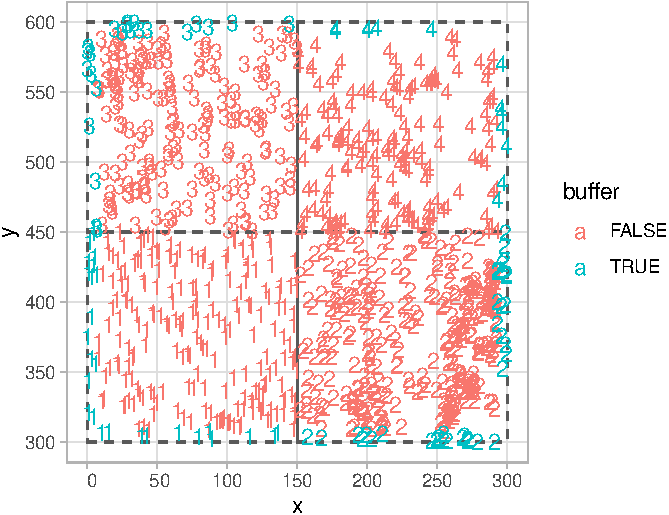
\includegraphics[width=0.66\linewidth]{Figures/scbi-spatial-information-1} 

}

\caption{Add spatial information: Buffer region and spatial cross-validation blocks (1 through 4). All trees in the interior of the study region (i.e. not part of buffer) will be the focal trees whose growth will be modeled.}\label{fig:scbi-spatial-information}
\end{figure}

\hypertarget{focal-vs-comp}{%
\subsection{Step 3: Identify all focal and corresponding competitor
trees}\label{focal-vs-comp}}

The next step in our analysis sequence is to identify all focal trees
and their corresponding competitor trees. More specifically, it
identifies all trees that are not part of the buffer region, have a
valid \texttt{growth} measurement, and have at least one neighbor within
7.5 of it. The \texttt{create\_focal\_vs\_comp()} functions performs
these tasks and returns a new data frame of type \texttt{sf}. On top of
the previous arguments \texttt{comp\_dist} defining the competition
neighborhood and \texttt{id} indicating which variable uniquely
identifies each tree-stem, this function also requires an \texttt{sf}
object representation of the spatial cross-validation blocks/folds. In
this example, the blocks were manually encoded in \texttt{blocks\_scbi}
by specifying it's vertices in Section
\ref{spatial-information}\footnote{We present an alternative method for
  defining spatial cross-validation blocks is using the
  \texttt{spatialBlock()} function from the \texttt{blockCV} package in
  the Supporting Information.}. We present the resulting data frame
below with the \texttt{foldID} variable omitted for compactness of
presentation.

\begin{Shaded}
\begin{Highlighting}[]
\NormalTok{focal_vs_comp_scbi <-}\StringTok{ }\NormalTok{growth_scbi }\OperatorTok
\StringTok{  }\KeywordTok{create_focal_vs_comp}\NormalTok{(comp_dist, }\DataTypeTok{blocks =}\NormalTok{ blocks_scbi, }\DataTypeTok{id =} \StringTok{"stemID"}\NormalTok{)}
\NormalTok{focal_vs_comp_scbi }\OperatorTok\StringTok{ }
\StringTok{  }\KeywordTok{select}\NormalTok{(}\OperatorTok{-}\NormalTok{foldID)}
\CommentTok{## # A tibble: 6,296 x 6}
\CommentTok{##   focal_ID focal_sp   dbh   geometry growth comp             }
\CommentTok{##      <dbl> <fct>    <dbl>    <POINT>  <dbl> <list>           }
\CommentTok{## 1        4 nysy     13.6  (14.2 428)  0.103 <tibble [20 x 4]>}
\CommentTok{## 2        5 havi      8.8   (9.4 436)  0.150 <tibble [32 x 4]>}
\CommentTok{## 3       79 tiam     47.7    (40 381) -0.161 <tibble [20 x 4]>}
\CommentTok{## 4       80 caca      5.15 (38.7 422)  0.253 <tibble [12 x 4]>}
\CommentTok{## 5       96 libe      2.3    (60 310)  0.262 <tibble [14 x 4]>}
\CommentTok{## # ... with 6,291 more rows}
\end{Highlighting}
\end{Shaded}

The resulting data frame \texttt{focal\_vs\_comp\_scbi} has 6296 rows,
representing the subset of the 7954 trees in \texttt{growth\_scbi} that
will be considered as focal trees. Two new variables \texttt{focal\_ID}
and \texttt{focal\_sp} relate to tree-stem identification and species
information. Most notably however is a new variable \texttt{comp} which
contains information on all competitor trees for a given focal tree,
saved in \texttt{tidyr} package list-column format
\citep{tidyr_package}. For example, we drill-down on the tree with
\texttt{focal\_ID} 4, which has 20 competitor trees each described by 4
variables as indicated by the fact that \texttt{comp} is a
\texttt{tibble\ {[}20\ ×\ 4{]}}.

\begin{Shaded}
\begin{Highlighting}[]
\NormalTok{focal_vs_comp_scbi }\OperatorTok\StringTok{ }
\StringTok{  }\KeywordTok{filter}\NormalTok{(focal_ID }\OperatorTok{==}\StringTok{ }\DecValTok{4}\NormalTok{) }\OperatorTok\StringTok{ }
\StringTok{  }\KeywordTok{select}\NormalTok{(focal_ID, dbh, comp)}
\CommentTok{## # A tibble: 1 x 3}
\CommentTok{##   focal_ID   dbh comp             }
\CommentTok{##      <dbl> <dbl> <list>           }
\CommentTok{## 1        4  13.6 <tibble [20 x 4]>}
\end{Highlighting}
\end{Shaded}

The spatial distribution of these trees is visualized in Figure
\ref{fig:scbi-focal-vs-comp-map}: the dashed circle extends 7.5 m away
from the focal tree while all 20 competitor trees are within this
circle.

\begin{figure}

{\centering 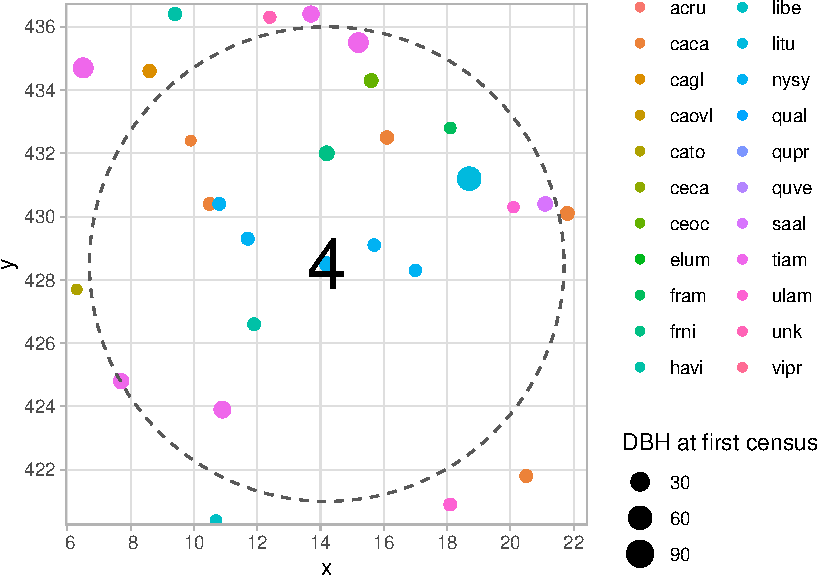
\includegraphics[width=0.66\linewidth]{Figures/scbi-focal-vs-comp-map-1} 

}

\caption{Identify all focal and corresponding competitor trees: All 20 competitor trees of focal tree 4.}\label{fig:scbi-focal-vs-comp-map}
\end{figure}

Using the \texttt{unnest()} function from the \texttt{tidyr} package, we
can flatten list-column into regular columns. We observe that for the
same focal tree, we have information on all 20 competitor trees whose
\texttt{dist} distance to the focal tree is \(\leq\) 7.5: their unique
tree-stem ID number, their species, and their basal area (in m\(^2\))
calculated as \(\frac{\pi \times (\text{DBH/2})^2}{10000}\) where
\(DBH\) is the value from the earlier of the two censuses in cm. Saving
our focal versus competitor information in list-column minimizes
redundancy since we do not repeat information on the focal tree 20
times.

\begin{Shaded}
\begin{Highlighting}[]
\NormalTok{focal_vs_comp_scbi }\OperatorTok\StringTok{ }
\StringTok{  }\KeywordTok{filter}\NormalTok{(focal_ID }\OperatorTok{==}\StringTok{ }\DecValTok{4}\NormalTok{) }\OperatorTok\StringTok{ }
\StringTok{  }\KeywordTok{select}\NormalTok{(focal_ID, dbh, comp) }\OperatorTok\StringTok{ }
\StringTok{  }\KeywordTok{unnest}\NormalTok{(}\DataTypeTok{cols =} \StringTok{"comp"}\NormalTok{)}
\CommentTok{## # A tibble: 20 x 6}
\CommentTok{##   focal_ID   dbh comp_ID  dist comp_sp comp_basal_area}
\CommentTok{##      <dbl> <dbl>   <dbl> <dbl> <fct>             <dbl>}
\CommentTok{## 1        4  13.6    1836  7.48 tiam            0.0176 }
\CommentTok{## 2        4  13.6    1847  2.81 nysy            0.00332}
\CommentTok{## 3        4  13.6    1848  1.62 nysy            0.00396}
\CommentTok{## 4        4  13.6    1849  2.62 nysy            0.00535}
\CommentTok{## 5        4  13.6    1850  2.98 havi            0.00472}
\CommentTok{## # ... with 15 more rows}
\end{Highlighting}
\end{Shaded}

\hypertarget{model-fit-predict}{%
\subsection{Step 4: Fit model}\label{model-fit-predict}}

Now that we've identified all focal and corresponding competitor trees
and saved this information in a data frame of type
\texttt{focal\_vs\_comp}, the final step in our analysis sequence is to
fit a model for the growth of all focal trees. Currently the
\texttt{forestecology} package can only fit the competition Bayesian
linear regression model outlined in Section \ref{competition-model}
using the \texttt{comp\_bayes\_lm()} function. However, any model
implemented in a function that similarly takes an input data frame of
type \texttt{focal\_vs\_comp} as an argument can also be used. For our
specific competition Bayesian linear regression model, we also specify
prior distributions on all parameters of interest (here chosen to be the
defaults as specified in \texttt{?comp\_bayes\_lm}).

\begin{Shaded}
\begin{Highlighting}[]
\NormalTok{comp_bayes_lm_scbi <-}\StringTok{ }\NormalTok{focal_vs_comp_scbi }\OperatorTok
\StringTok{  }\KeywordTok{comp_bayes_lm}\NormalTok{(}\DataTypeTok{prior_param =} \OtherTok{NULL}\NormalTok{)}
\end{Highlighting}
\end{Shaded}

The returned \texttt{comp\_bayes\_lm\_scbi} output is an object of S3
class type \texttt{comp\_bayes\_lm} which contains the posterior values
of all parameters in our competition Bayesian linear regression. This
class of object includes generic methods implemented for
\texttt{print()}, \texttt{predict()}, and \texttt{ggplot2::autoplot()}.
First the generic for \texttt{print()} displays the names of all prior
\& posterior parameters along with the model formula:

\begin{Shaded}
\begin{Highlighting}[]
\NormalTok{comp_bayes_lm_scbi}
\CommentTok{## Bayesian linear regression model parameters with a multivariate Normal likelihood. See ?comp_bayes_lm for details:}
\CommentTok{## }
\CommentTok{##   parameter_type           prior posterior}
\CommentTok{## 1 Inverse-Gamma on sigma^2 a_0   a_star   }
\CommentTok{## 2 Inverse-Gamma on sigma^2 b_0   b_star   }
\CommentTok{## 3 Multivariate t on beta   mu_0  mu_star  }
\CommentTok{## 4 Multivariate t on beta   V_0   V_star   }
\CommentTok{## }
\CommentTok{## Model formula:}
\CommentTok{## growth ~ sp + dbh + dbh * sp + acne * sp + acru * sp + amar * sp + astr * sp + caca * sp + caco * sp + cade * sp + cagl * sp + caovl * sp + cato * sp + ceca * sp + ceoc * sp + chvi * sp + cofl * sp + crpr * sp + crsp * sp + divi * sp + elum * sp + fagr * sp + fram * sp + frni * sp + frpe * sp + havi * sp + ilve * sp + juci * sp + juni * sp + libe * sp + litu * sp + nysy * sp + pist * sp + pivi * sp + ploc * sp + prav * sp + prse * sp + qual * sp + quco * sp + qufa * sp + qumi * sp + qupr * sp + quru * sp + quve * sp + rops * sp + saal * sp + saca * sp + tiam * sp + ulam * sp + ulru * sp + unk * sp + vipr * sp}
\end{Highlighting}
\end{Shaded}

Next, the generic for \texttt{predict()} takes as inputs the posterior
parameter values in \texttt{comp\_bayes\_lm\_scbi} and the predictor
variables in \texttt{newdata} and outputs a vector of fitted/predicted
values \(\widehat{y}\) of the DBH for each focal tree computed from the
posterior predictive distribution.

\begin{Shaded}
\begin{Highlighting}[]
\NormalTok{focal_vs_comp_scbi <-}\StringTok{ }\NormalTok{focal_vs_comp_scbi }\OperatorTok
\StringTok{  }\KeywordTok{mutate}\NormalTok{(}\DataTypeTok{growth_hat =} \KeywordTok{predict}\NormalTok{(comp_bayes_lm_scbi, }\DataTypeTok{newdata =}\NormalTok{ focal_vs_comp_scbi))}
\end{Highlighting}
\end{Shaded}

\begin{Shaded}
\begin{Highlighting}[]
\NormalTok{focal_vs_comp_scbi}
\CommentTok{## # A tibble: 6,296 x 8}
\CommentTok{##   focal_ID focal_sp   dbh foldID                  geometry growth comp }
\CommentTok{##      <dbl> <fct>    <dbl> <fct>                    <POINT>  <dbl> <lis>}
\CommentTok{## 1        4 nysy     13.6  1                     (14.2 428)  0.103 <tib~}
\CommentTok{## 2        5 havi      8.8  1                      (9.4 436)  0.150 <tib~}
\CommentTok{## 3       79 tiam     47.7  1                       (40 381) -0.161 <tib~}
\CommentTok{## 4       80 caca      5.15 1                     (38.7 422)  0.253 <tib~}
\CommentTok{## 5       96 libe      2.3  1                       (60 310)  0.262 <tib~}
\CommentTok{## # ... with 6,291 more rows, and 1 more variable: growth_hat <dbl>}
\end{Highlighting}
\end{Shaded}

We then compare the observed and fitted/predicted growths to compute the
root mean squared error (RMSE) of our model fit.

\begin{Shaded}
\begin{Highlighting}[]
\NormalTok{model_rmse <-}\StringTok{ }\NormalTok{focal_vs_comp_scbi }\OperatorTok
\StringTok{  }\KeywordTok{rmse}\NormalTok{(}\DataTypeTok{truth =}\NormalTok{ growth, }\DataTypeTok{estimate =}\NormalTok{ growth_hat) }\OperatorTok
\StringTok{  }\KeywordTok{pull}\NormalTok{(.estimate)}
\NormalTok{model_rmse}
\CommentTok{## [1] 0.128}
\end{Highlighting}
\end{Shaded}

Lastly, the generic for \texttt{ggplot2::autoplot()} allows us to plot
the posterior distribution of all parameters in Figure
\ref{fig:scbi-posterior-viz} (for compactness we only show posteriors
for 3 species).

\begin{Shaded}
\begin{Highlighting}[]
\CommentTok{# Plot posteriors for only a subset of species}
\NormalTok{sp_to_plot <-}\StringTok{ }\KeywordTok{c}\NormalTok{(}\StringTok{"litu"}\NormalTok{, }\StringTok{"quru"}\NormalTok{, }\StringTok{"cagl"}\NormalTok{)}

\NormalTok{plot1 <-}\StringTok{ }\KeywordTok{autoplot}\NormalTok{(comp_bayes_lm_scbi, }\DataTypeTok{type =} \StringTok{"intercepts"}\NormalTok{, }
                  \DataTypeTok{sp_to_plot =}\NormalTok{ sp_to_plot)}
\NormalTok{plot2 <-}\StringTok{ }\KeywordTok{autoplot}\NormalTok{(comp_bayes_lm_scbi, }\DataTypeTok{type =} \StringTok{"dbh_slopes"}\NormalTok{, }
                  \DataTypeTok{sp_to_plot =}\NormalTok{ sp_to_plot)}
\NormalTok{plot3 <-}\StringTok{ }\KeywordTok{autoplot}\NormalTok{(comp_bayes_lm_scbi, }\DataTypeTok{type =} \StringTok{"competition"}\NormalTok{, }
                  \DataTypeTok{sp_to_plot =}\NormalTok{ sp_to_plot)}

\CommentTok{# Combine plots using patchwork}
\NormalTok{(plot1 }\OperatorTok{|}\StringTok{ }\NormalTok{plot2) }\OperatorTok{/}\StringTok{ }\NormalTok{plot3}
\end{Highlighting}
\end{Shaded}

\begin{figure}

{\centering 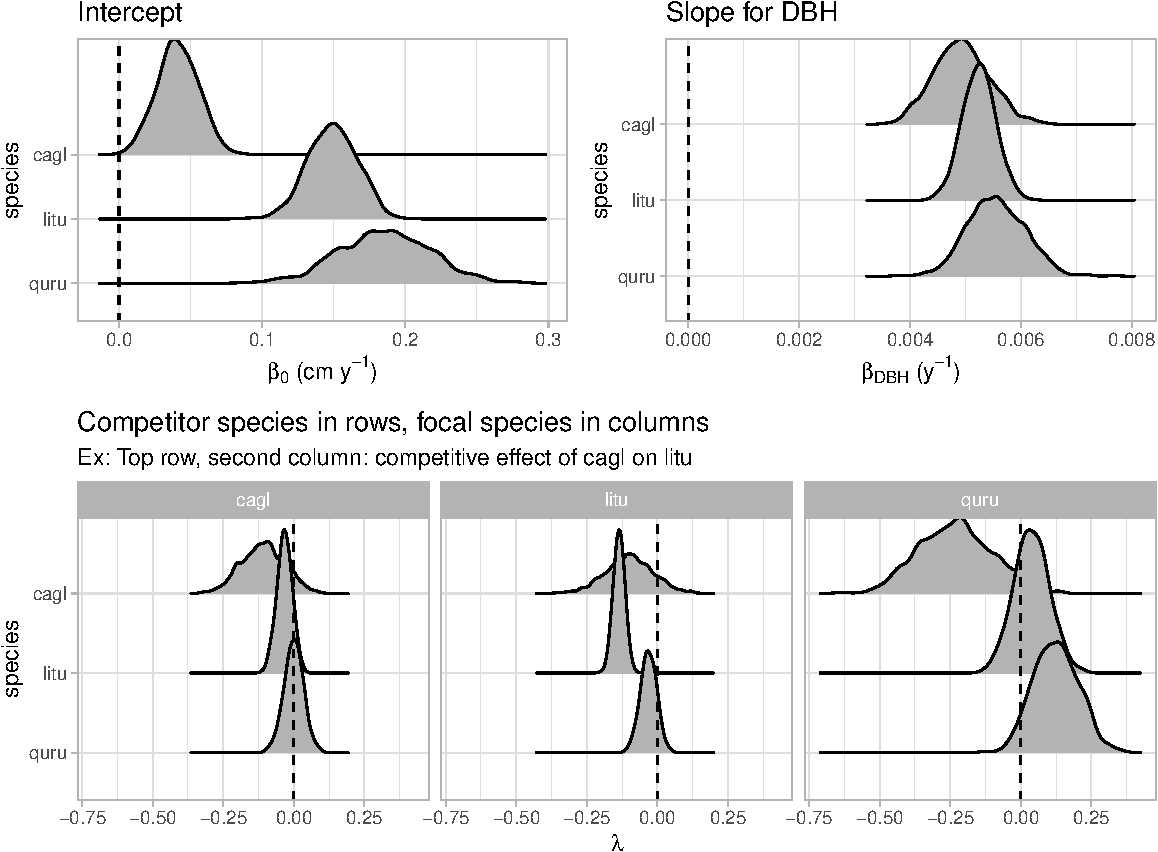
\includegraphics[width=1\linewidth]{Figures/scbi-posterior-viz-1} 

}

\caption{Fit model: Posterior distributions of all parameters for three species.}\label{fig:scbi-posterior-viz}
\end{figure}

These plots give the posterior distributions of parameters from Equation
\ref{eq:model}. For many package users they will be of interest because
they give insight into the species-specific competitive interactions.
Setting \texttt{type\ =\ "intercepts"} gives posterior distributions for
\(\beta_{0,j}\) and \texttt{type\ =\ "dbh\_slopes"} for
\(\beta_{dbh,j}\). These give species specific growth independent of
competition. The values of more interest are plotted with
\texttt{type\ =\ \textquotesingle{}competition\textquotesingle{}} which
gives the posterior distribution for \(\lambda_{j,k}\) species-specific
competition coefficients (i.e., the \(\lambda\)-matrix). Negative values
indicate a competitor species which slows the growth of a focal species.
Here, for example, we see that tulip trees (\texttt{litu}) have a strong
negative effect on the growth of conspecifics but relatively little
effect on neighbors of the other two species.

\hypertarget{evaluate-the-effect-of-competitor-species-identity-using-permutation-tests}{%
\subsection{Evaluate the effect of competitor species identity using
permutation
tests}\label{evaluate-the-effect-of-competitor-species-identity-using-permutation-tests}}

In order to evaluate the effect of competitor species identity, we use
the four steps of our analysis sequence answer along with a permutation
test: Under a null hypothesis where competitor species identity does not
matter, we can permute/shuffle this variable within each focal tree,
compute the RMSE (the test statistic of interest), repeat this process
several times to construct a null distribution of the RMSE, and compare
it to the observed RMSE to assess significance. Going back to our
example in Section \ref{focal-vs-comp} of focal tree with
\texttt{focal\_ID} 4 and its 20 competitors, the permutation test
randomly resamples the \texttt{comp\_sp} variable with replacement,
leaving all other variables intact. The resampling with replacement is
nested within each focal tree in order to preserve the neighborhood
structure of our competition model. To run the permutation test, we use
the same \texttt{comp\_bayes\_lm()} function as in Section
\ref{model-fit-predict}, but with a \texttt{run\_shuffle\ =\ TRUE}
argument.

\begin{Shaded}
\begin{Highlighting}[]
\NormalTok{comp_bayes_lm_scbi_shuffle <-}\StringTok{ }\NormalTok{focal_vs_comp_scbi }\OperatorTok
\StringTok{  }\KeywordTok{comp_bayes_lm}\NormalTok{(}\DataTypeTok{prior_param =} \OtherTok{NULL}\NormalTok{, }\DataTypeTok{run_shuffle =} \OtherTok{TRUE}\NormalTok{)}

\NormalTok{focal_vs_comp_scbi <-}\StringTok{ }\NormalTok{focal_vs_comp_scbi }\OperatorTok
\StringTok{  }\KeywordTok{mutate}\NormalTok{(}
    \DataTypeTok{growth_hat_shuffle =} \KeywordTok{predict}\NormalTok{(comp_bayes_lm_scbi_shuffle, }
                                 \DataTypeTok{newdata =}\NormalTok{ focal_vs_comp_scbi)}
\NormalTok{  )}
\end{Highlighting}
\end{Shaded}

\begin{Shaded}
\begin{Highlighting}[]
\NormalTok{model_rmse_shuffle <-}\StringTok{ }\NormalTok{focal_vs_comp_scbi }\OperatorTok
\StringTok{  }\KeywordTok{rmse}\NormalTok{(}\DataTypeTok{truth =}\NormalTok{ growth, }\DataTypeTok{estimate =}\NormalTok{ growth_hat_shuffle) }\OperatorTok
\StringTok{  }\KeywordTok{pull}\NormalTok{(.estimate)}
\NormalTok{model_rmse_shuffle}
\CommentTok{## [1] 0.131}
\end{Highlighting}
\end{Shaded}

The resulting RMSE of 0.131 based on the permutation test is larger than
the earlier RMSE of 0.128, suggesting that models that do incorporate
competitor species identity better fit the data.

\hypertarget{spatial-cross-validation}{%
\subsection{Evaluate model performance using spatial
cross-validation}\label{spatial-cross-validation}}

We answer the second of our two questions: how can we obtain an accurate
estimate of model performance/error? The model fits and predictions in
Section \ref{model-fit-predict} all suffer from a common failing: they
use the same data to both fit the model and to assess the model's
performance using the RMSE. As argued by
\citet{roberts_cross-validation_2017}, this can lead to overly
optimistic assessments of model quality as the models can be overfit, in
particular in situations where spatial-autocorrelation is present. To
mitigate the effects of such overfitting, we use a spatially block
cross-validation algorithm.

To this end, we use the \texttt{foldID} variable defined in Section
\ref{spatial-information} whereby all focal trees are assigned to one of
4 spatially contiguous blocks that act as folds in our cross-validation
routine. Figure \ref{fig:scbi-spatial-cross-validation-schematic}
presents a schematic illustrating this scheme for fold 1 (bottom-left)
as the test set and folds 2, 3, and 4 as the training sets. We fit the
model to all focal trees in the training set, apply the model to all
focal trees in the test set to compute fitted/predicted values, and
compute the RMSE of the observed versus predicted growths. We repeat
this procedure 3 more times with each of the three remaining folds
acting as the test set and then average all four resulting RMSE's.
Furthermore, in order to maintain spatial independence between the test
and training set, a fold buffer that extend outwards from the boundary
of the test set is computed; all trees falling within this fold buffer
are excluded from the training set.

\begin{figure}

{\centering 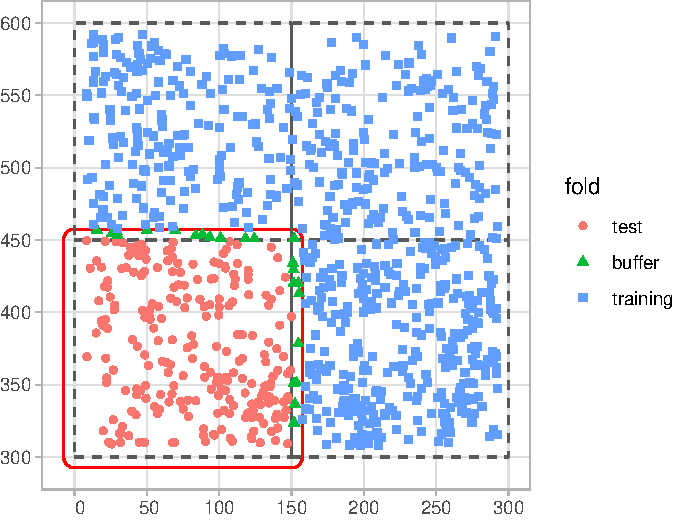
\includegraphics[width=0.66\linewidth]{Figures/scbi-spatial-cross-validation-schematic-1} 

}

\caption{Schematic of spatial cross-validation: Using the k = 1 fold as the test set, assigning each focal tree to training set, test set, and fold buffer.}\label{fig:scbi-spatial-cross-validation-schematic}
\end{figure}

This algorithm is implemented in the \texttt{run\_cv()} function, which
is a wrapper function to the \texttt{comp\_bayes\_lm()} function that
fits the model and the \texttt{predict()} generic that returns
fitted/predicted values. We compare these values to the observed growth
values to again compute our RMSE.

\begin{Shaded}
\begin{Highlighting}[]
\NormalTok{focal_vs_comp_scbi <-}\StringTok{ }\NormalTok{focal_vs_comp_scbi }\OperatorTok
\StringTok{  }\KeywordTok{run_cv}\NormalTok{(}\DataTypeTok{comp_dist =}\NormalTok{ comp_dist, }\DataTypeTok{blocks =}\NormalTok{ blocks_scbi)}
\end{Highlighting}
\end{Shaded}

\begin{Shaded}
\begin{Highlighting}[]
\NormalTok{model_rmse_cv <-}\StringTok{ }\NormalTok{focal_vs_comp_scbi }\OperatorTok
\StringTok{  }\KeywordTok{rmse}\NormalTok{(}\DataTypeTok{truth =}\NormalTok{ growth, }\DataTypeTok{estimate =}\NormalTok{ growth_hat) }\OperatorTok
\StringTok{  }\KeywordTok{pull}\NormalTok{(.estimate)}
\NormalTok{model_rmse_cv}
\CommentTok{## [1] 0.14}
\end{Highlighting}
\end{Shaded}

The resulting RMSE of 0.14 computed using cross-validation is larger
than the earlier RMSE of 0.128, suggesting that models that do not take
the inherent spatial autocorrelation of the data into account generate
error estimates that are overly optimistic; in our case RMSE's that are
too low.

\hypertarget{importance-of-spatial-cross-validation}{%
\section{Importance of spatial cross
validation}\label{importance-of-spatial-cross-validation}}

The \texttt{run\_cv} function also accepts the \texttt{run\_shuffle}
argument. This permutes the competitor species, as described above, but
does so when calculating predicted growth with the cross validated
scheme. Figure \ref{fig:scbi-simulation} compares model performance when
permuting competitor species and calculating RMSE with and without cross
validation. Without cross-validation the competitor identity did matter,
the non-permuted competitor species had a much lower RMSE than the
permuted one. But once we include the spatial cross validation this
improvement disappears. So in this 9 ha subplot of the SCBI plot
competitive interactions do not depend on the identity of the
competitor, which is the opposite of what has been observed in other
places (\citet{allen_permutation_2020} \citet{uriarte_spatially_2004}).
This highlights the importance of cross validation, without it the model
was overfit.

\begin{figure}

{\centering 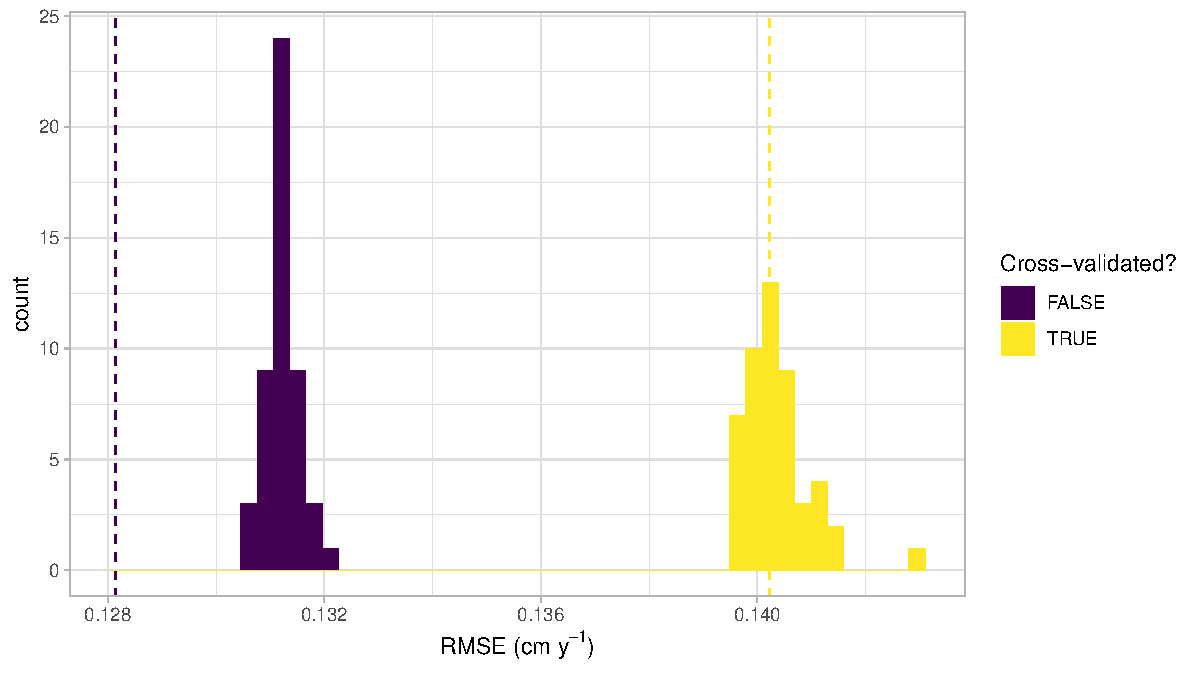
\includegraphics[width=1\linewidth]{simulation_results/2021-03-03_scbi_49_shuffles} 

}

\caption{Root mean squared error of models for standard, permuted, and spatial cross-validated error estimates. The dotted lines show non-permuted competitor identity, while the histogras so the RMSE for 49 permutations. The colors indicate whether cross validaton was used.}\label{fig:scbi-simulation}
\end{figure}

\hypertarget{conclusion}{%
\section{Conclusion}\label{conclusion}}

The \texttt{forestecology} package provides an accessible way to fit and
test models of neighborhood competition. Currently it is written to work
with data from ForestGEO plots. But it could easily be modified to work
on any single large, mapped forest plot in which at least two
measurements of each individual have been taken. With a little bit of
work the package could also be applied to forest inventory data in which
several small plots are spatially separated, e.g., USFS Forest
Inventory. In a future version of the package we also hope to make it
possible to model plant mortality in addition to plant growth. The
package follows the guidelines for \texttt{tidy} data, \texttt{sf}
spatial structure, and S3 open-oriented model structure. We hope that
the package will increase the use of neighborhood competition models to
better understand what structures plant competition.

\hypertarget{acknowledgments}{%
\section{Acknowledgments}\label{acknowledgments}}

The authors thank Ryan Giordano and Jonathan Che for their help with the
statistical methodology and Sophie Li for their feedback on package
interface. The authors declare no conflicts of interest.

\hypertarget{authors-contributions}{%
\section{Author's contributions}\label{authors-contributions}}

AYK and DNA conceived the ideas and coded a draft of the package. AYK
wrote an initial manuscript draft. SPC rewrote much of the package's
code to align with R and ``tidy'' best practices
\citep{wickham_welcome_2019}. All authors contributed to subsequent
drafts and gave final approval for manuscript.

\hypertarget{data-accessibility}{%
\section{Data accessibility}\label{data-accessibility}}

We intend to archive all data and source code for the
\texttt{forestecology} package as well as this manuscript on GitHub at
\url{https://github.com/rudeboybert/forestecology}. This repository will
be versioned and archived on Zenodo upon acceptance. The 2008 and 2014
Smithsonian Conservation Biology Institute census data loaded in Section
\ref{compute-growth} and saved in \texttt{scbi.stem2.csv} and
\texttt{scbi.stem3.csv} are available on GitHub at
\url{https://github.com/SCBI-ForestGEO/SCBI-ForestGEO-Data/tree/master/tree_main_census/data/census-csv-files}
and have been versioned and archived on Zenodo at
\url{https://doi.org/10.5281/zenodo.2649301}
\citep{gonzalez-akre_scbi-forestgeoscbi-forestgeo-data_2020}.

\bibliographystyle{agsm}
\bibliography{paper.bib}

\end{document}
